
%(BEGIN_QUESTION)
% Copyright 2012, Tony R. Kuphaldt, released under the Creative Commons Attribution License (v 1.0)
% This means you may do almost anything with this work of mine, so long as you give me proper credit

Calculate the mechanical advantage for this lever system:

$$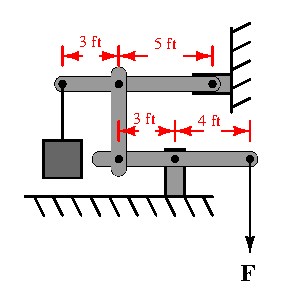
\includegraphics[width=15.5cm]{i02619x01.eps}$$

\underbar{file i02619}
%(END_QUESTION)





%(BEGIN_ANSWER)

The first lever (where force {\bf F} works on the right-hand end) is a first-class, with a mechanical advantage of 4:3.  It connects to a second lever (third-class), with an mechanical advantage ratio (actually, a {\it disadvantage} ratio) of 5:8.  The overall mechanical advantage is the product of these two advantage ratios:

$$M_A = \left( 4 \over 3 \right) \left(5 \over 8 \right) = {5 \over 6} = 0.83333$$

In other words, for every pound of force applied at {\bf F}, there will be 0.8333 pounds of force available to move the mass.

%(END_ANSWER)





%(BEGIN_NOTES)


%INDEX% Machine, lever
%INDEX% Machine, mechanical advantage

%(END_NOTES)


